\section{GRASS Integration}\label{sec:grass}\index{GRASS}

The GRASS~\cite{GRASSweb} plugin provides access to GRASS from within QGIS. 
This includes the ability to view, edit, and create data, as well as perform 
analysis using the GRASS geoprocessing modules.

In this chapter we'll introduce the plugin and some of the ways you can use 
it to work with GRASS data. The following features are provided with the GRASS 
plugin:
 
\begin{itemize}
\item 
\includegraphics[width=0.7cm]{add_grass_vector} Add GRASS vector layers
\item 
\includegraphics[width=0.7cm]{add_grass_raster} Add GRASS raster layers
\item 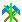
\includegraphics[width=0.7cm]{grass_tools} GRASS Toolbox
\item 
\includegraphics[width=0.7cm]{grass_region_edit} Changing the GRASS region
\item 
\includegraphics[width=0.7cm]{grass_edit} Vector layers digitizing
\item 
\includegraphics[width=0.7cm]{grass_open_mapset} Open existing mapset
\item 
\includegraphics[width=0.7cm]{grass_new_mapset} Create new GRASS mapset
\item 
\includegraphics[width=0.7cm]{grass_new_vector_layer} Create new GRASS
vector layer
\item 
\includegraphics[width=0.7cm]{grass_close_mapset} Close GRASS mapset
\end{itemize}

\subsection{Starting QGIS with GRASS}\label{sec:starting_grass}
\index{GRASS!starting QGIS}

To use GRASS features from within QGIS, you must load the 
GRASS plugin with the plugin manager (see Section \ref{sec:managing_plugins}) just 
like all QGIS plugins. After you load it, a new toolbar will appear on the user 
interface.\footnote{The GRASS plugin is unique in that it creates its own toolbar} 

After loading the plugin, you can immediately load an existing GRASS dataset 
using the appropriate toolbar buttons for vector and raster data (see Section 
\ref{sec:load_grassdata}), or you can create a new GRASS location with QGIS (see Section 
\ref{sec:create_loc}).

\subsection{Loading GRASS Data}\label{sec:load_grassdata}\index{GRASS!loading data}

With the GRASS plugin, you can load vector or raster layer using the appropriate button 
on the toolbar. As an example we use the spearfish sample location in UTM projection 
(see Section \ref{label_sampledata}).

\begin{enumerate}
  \item Download the spearfish\_grass60data-0.3.zip file
  \item Create a new folder \textsl{grassdata} and unzip the spearfish\_grass60data-0.3.zip into it. 
  \item Start QGIS
  \item In the GRASS toolbar, click on the \textsl{Open mapset} icon to bring 
  up the \textsl{Select GRASS mapset} wizard.
  \item For \textsl{Gisdbase} browse and enter the path to the newly created folder \textsl{grassdata}.
  \item You should now be able to select the location \textsl{spearfish60} and the mapset 
  \textsl{PERMANENT} or \textsl{user1}. 
  \item Click \textsl{OK}. Notice that some of the tools in the GRASS toolbar that were 
  disabled are now enabled.
  \item Click on \textsl{Add GRASS raster layer}, choose the \textsl{map name} geology and click 
  \textsl{OK}. The geology map will be visualized. 
  \item Click on \textsl{Add GRASS vector layer}, choose the \textsl{map name} roads and click 
  \textsl{OK}. Now the roads map will be overlayed on top of the geology.  
\end{enumerate}

As you see, it is very simple to load GRASS raster and vector layers in QGIS. See following sections 
for editing GRASS data and creating new locations.

\begin{Tip}\caption{\textsc{GRASS Data Loading}}
\qgistip{If you have problems loading data or QGIS terminates abnormally,
check to make sure you have loaded the GRASS plugin properly as described in Section
\ref{sec:starting_grass}.
}
\end{Tip} 

\subsection{Creating a Location}\label{sec:create_loc}

GRASS stores data in a ``location'' which represents a specific area with a 
specific coordinate system. In order to use GRASS data, we must import it 
into a \textsl{location}.\footnote{This is not strictly true - you can 
view external data sets without importing them}

\begin{figure}[ht]
   \begin{center}
   \caption{Creating a GRASS location in QGIS}\label{fig:grass_location}\smallskip
   
\includegraphics[clip=true, width=8cm]{grass_location}
\end{center}  
\end{figure}

Here is an example how to create a GRASS location in Albers Equal Area 
projection with unit meter for the QGIS sample data (see Section \ref{label_sampledata}). 

\begin{enumerate}
  \item Start QGIS
  \item Make sure the GRASS plugin is loaded
  \item Load the \textsl{alaska.shp} shapefile (see Section \ref{sec:load_shapefile}).
  \item In the GRASS toolbar, click on the \textsl{New mapset} tool to bring 
  up the mapset wizard
  \item Each location is stored in a directory. Select an existing data 
  directory or create a new one for storing the location
  \item Click \textsl{Next} 
  \item We can use this wizard to create a new mapset within an existing 
  location or create a new location altogether. Click ``Create new location'' 
  radio button
  \item Enter a name for the location - we'll use Alaska
  \item Click \textsl{Next} 
  \item Define the projection by clicking on the ``Projection'' radio button 
  to enable the projection list
  \item We are using Albers Equal Area Alaska (meters) projection. Since we happen to know that 
  its PostGIS SRID is 5000, we enter it in the search box. (If you want to repeat this process 
  for another layer and haven't memorized the PostGIS SRID, click on the projector icon in the 
  lower right-hand corner of the statusbar (see Section \ref{label_projstart}).)
  \item Click \textsl{Find} to select the projection
  \item Click \textsl{Next} 
  \item To define the default region, we have to enter the bounds in the north, south, 
  east, and west direction. Here we simply click on the button \textsl{Set current QGIS extent}.
  \item Click \textsl{Next} 
  \item We need to define a mapset within our new location. Name it whatever 
  you like - your username is a good choice
  \item Check out the summary to make sure it's correct
  \item Click \textsl{Finish} 
  \item The mapset and location are created and opened as the current 
  working set
  \item Notice that some of the tools in the GRASS toolbar that were 
  disabled are now enabled for us to use
\end{enumerate}

If that seemed like a lot of steps, it's really not all that bad and a very 
quick way to create a location. Our location is now ready for use. To view 
the default region, zoom out. Clicking the \textsl{Display Current Grass Region} tool 
toggles the display region on and off. 

\subsection{Vector Data Model}\label{label_vectmodel}\index{GRASS!vector data
model}

It is important to understand the GRASS vector data model prior to
digitizing.\index{GRASS!digitizing} In general, GRASS uses a topological
vector model.\index{GRASS!topology} This means that areas are not represented
as closed polygons, but by one or more boundaries. A boundary between two
adjacent areas is digitized only once, and it is shared by both areas.
Boundaries must be connected without gaps. An area is identified (labeled) by
the centroid of the area.

Besides boundaries and centroids, a vector map can also contain
points and lines. All these geometry elements can be mixed
in one vector and will be represented in different so called 'layers' inside
QGIS.

It is possible to store more 'layers' in one vector dataset. For example,
fields, forests and lakes can be stored in one vector. Adjacent
forest and lake can share the same boundary, but they have separate attribute
tables. It is also possible to attach attributes to boundaries. For example,
the boundary between lake and forest is a road, so it can have a different 
attribute table.
 
The 'layer' of the feature is defined by 'layer' inside GRASS.
'Layer' is the number which defines if there are more than one layer inside the 
dataset, e.g. if the geometry is forest or lake.
For now, it can be only a number, in the future GRASS will also support  
names as fields in the user interface.

Attributes can be stored in external database tables, for example
DBF, PostgreSQL, MySQL, SQLITE3, etc.\index{GRASS!attribute storage}

Attributes in database tables are linked to geometry elements using
'category'.\index{GRASS!attribute linkage} 'Category' (key, ID) is an
integer attached to geometry primitives, and it is used as the link to one
column in the database table.

\begin{Tip}\caption{\textsc{Learning the GRASS Vector Model}}
\qgistip{
The best way to learn the GRASS vector model and its capabilities is to 
download one of the many GRASS Tutorials where the vector model is described
more deeply. See \url{http://grass.itc.it/gdp/manuals.php} for more
information, books and tutorials in several languages.
}
\end{Tip} 

\subsection{Digitizing and Editing Tools}\index{GRASS!digitizing tools}
\label{grass_digitising}


\includegraphics[width=0.7cm]{grass_edit} The digitizing tools for GRASS vector layers are accessed using the
\textsl{Edit GRASS Vector Layer} tool on the toolbar. Make sure you have
loaded a GRASS vector and it is the selected layer in the legend before
clicking on the edit tool. If you would like to create a new GRASS vector, 
you need to use the toolbar-entry Plugins->GRASS->Create new GRASS vector layer

Figure \ref{fig:grass_edit} shows the GRASS Edit dialog that
is displayed when you click on the edit tool. 

\begin{figure}[h]
   \begin{center}
   \caption{GRASS Edit Dialog}\label{fig:grass_edit}\smallskip
   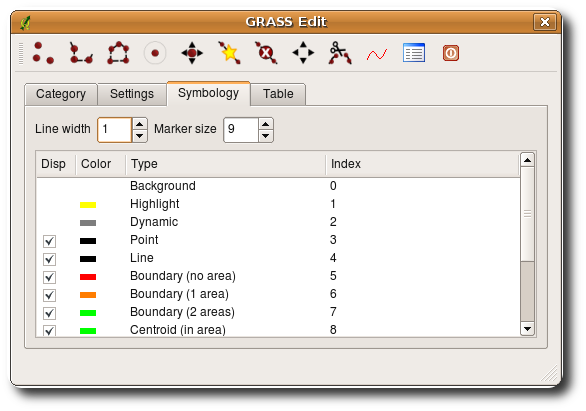
\includegraphics[clip=true, width=13cm]{grassedit}
\end{center}  
\end{figure}

The tools and settings are discussed in the following sections.

\subsubsection{Toolbar}\label{label_grasstoolbar}

Table \ref{tab:grass_tools} lists the digitizing tools provided by the GRASS
plugin. These correspond to the tool buttons in the toolbar(s) across the top
of the dialog.

\begin{table}[h]\index{GRASS!digitizing tools}
\centering
\caption{GRASS Digitizing Tools}\label{tab:grass_tools}\medskip
 \begin{tabular}{|l|l|p{5in}|}
 \hline \textbf{Icon} & \textbf{Tool} & \textbf{Purpose} \\
\hline 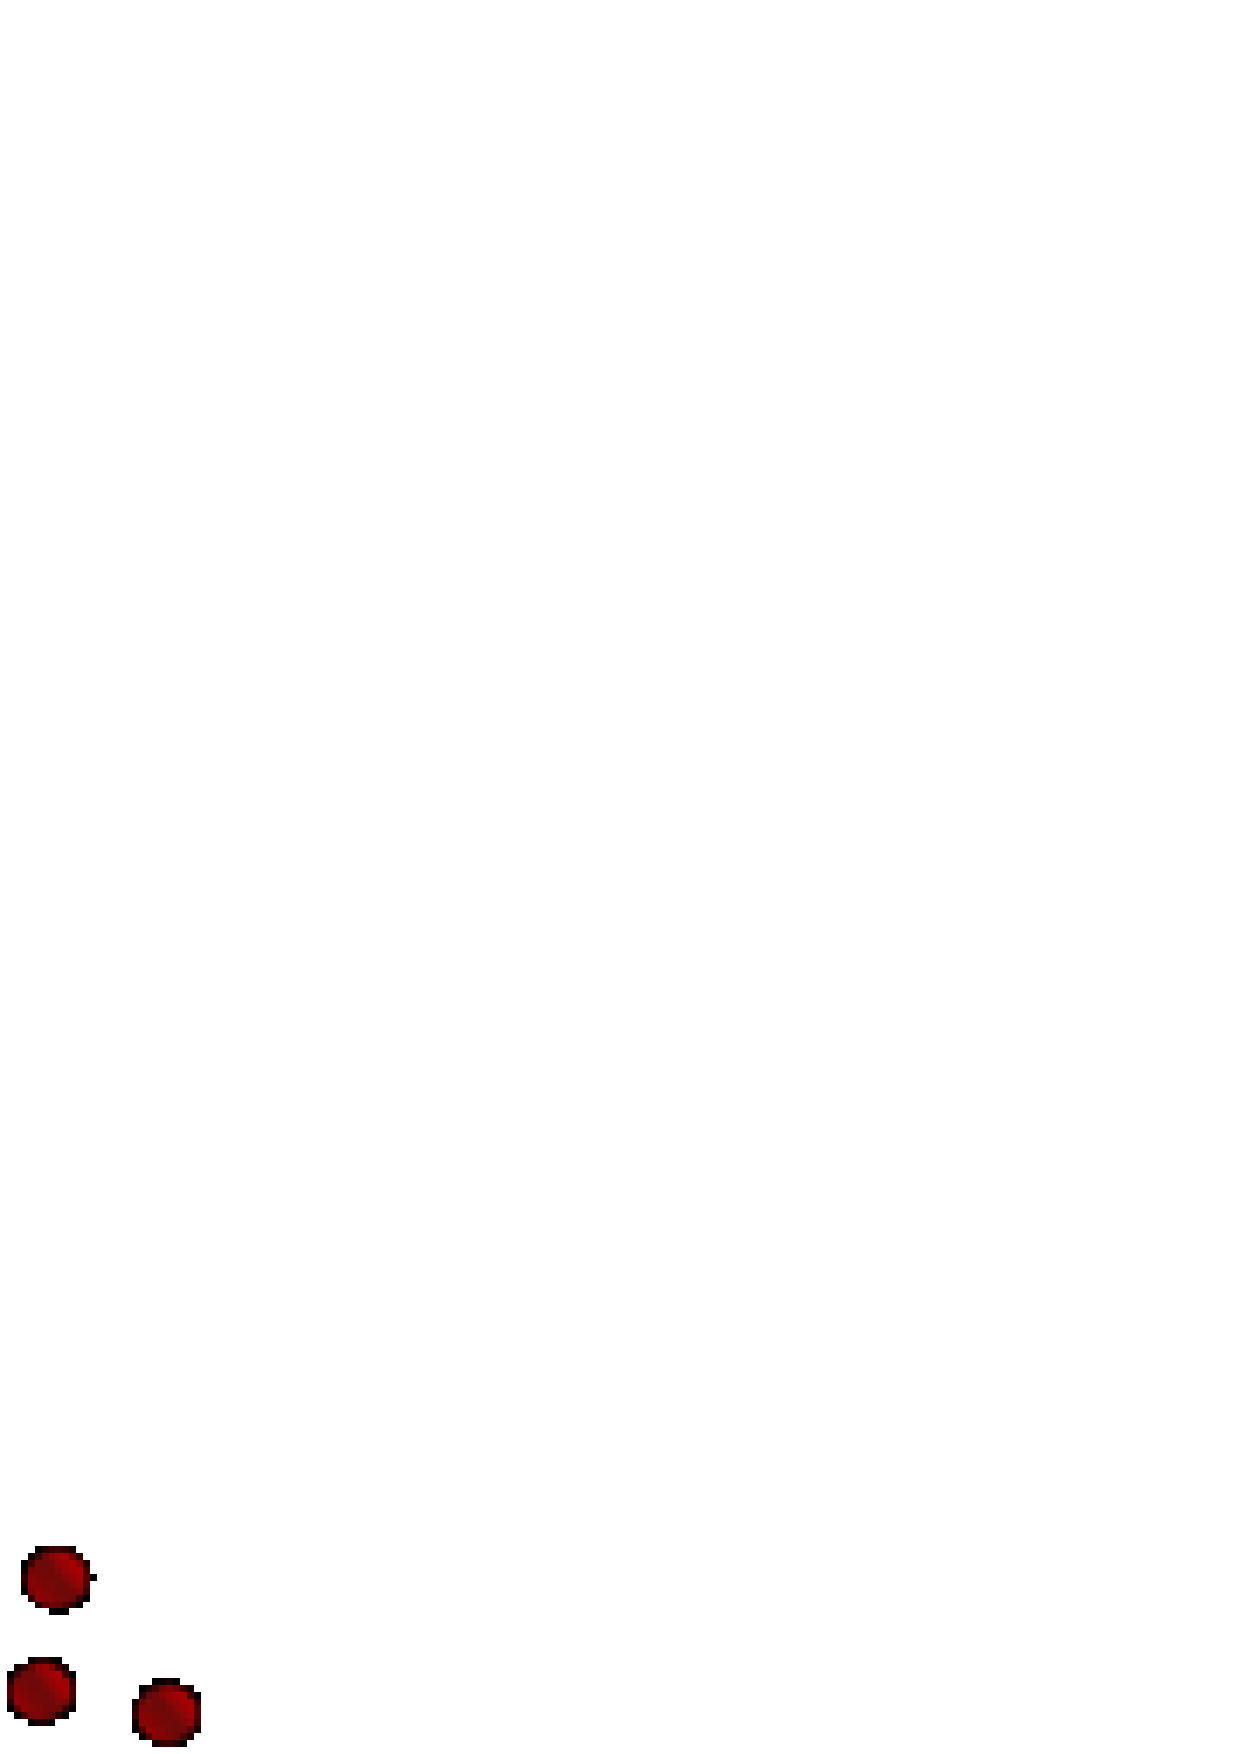
\includegraphics[width=0.7cm]{grass_new_point} & New Point & digitize new point \\
\hline 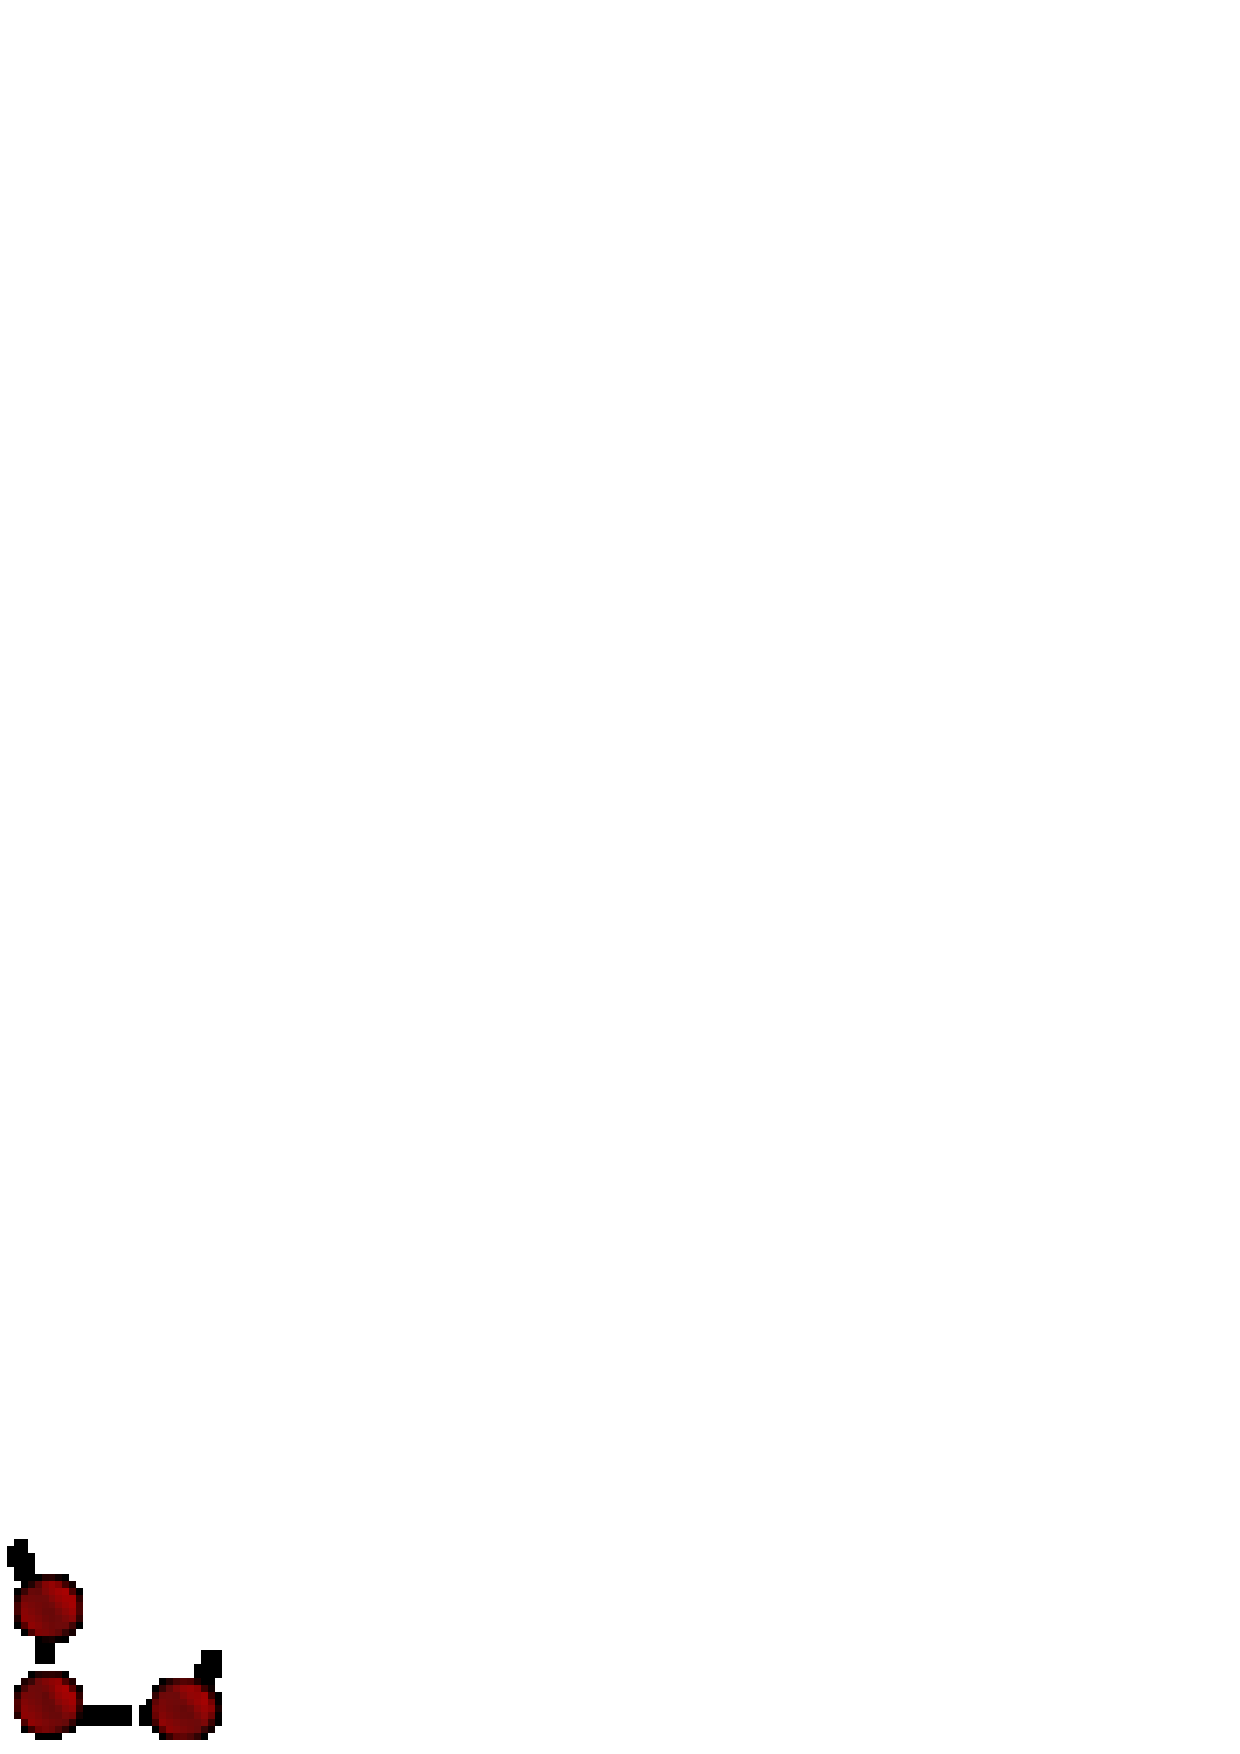
\includegraphics[width=0.7cm]{grass_new_line} & New Line &  digitize new line (finish by selecting new tool) \\
\hline 
\includegraphics[width=0.7cm]{grass_new_boundary} & New Boundary & digitize new boundary (finish by selecting new tool)\\
\hline 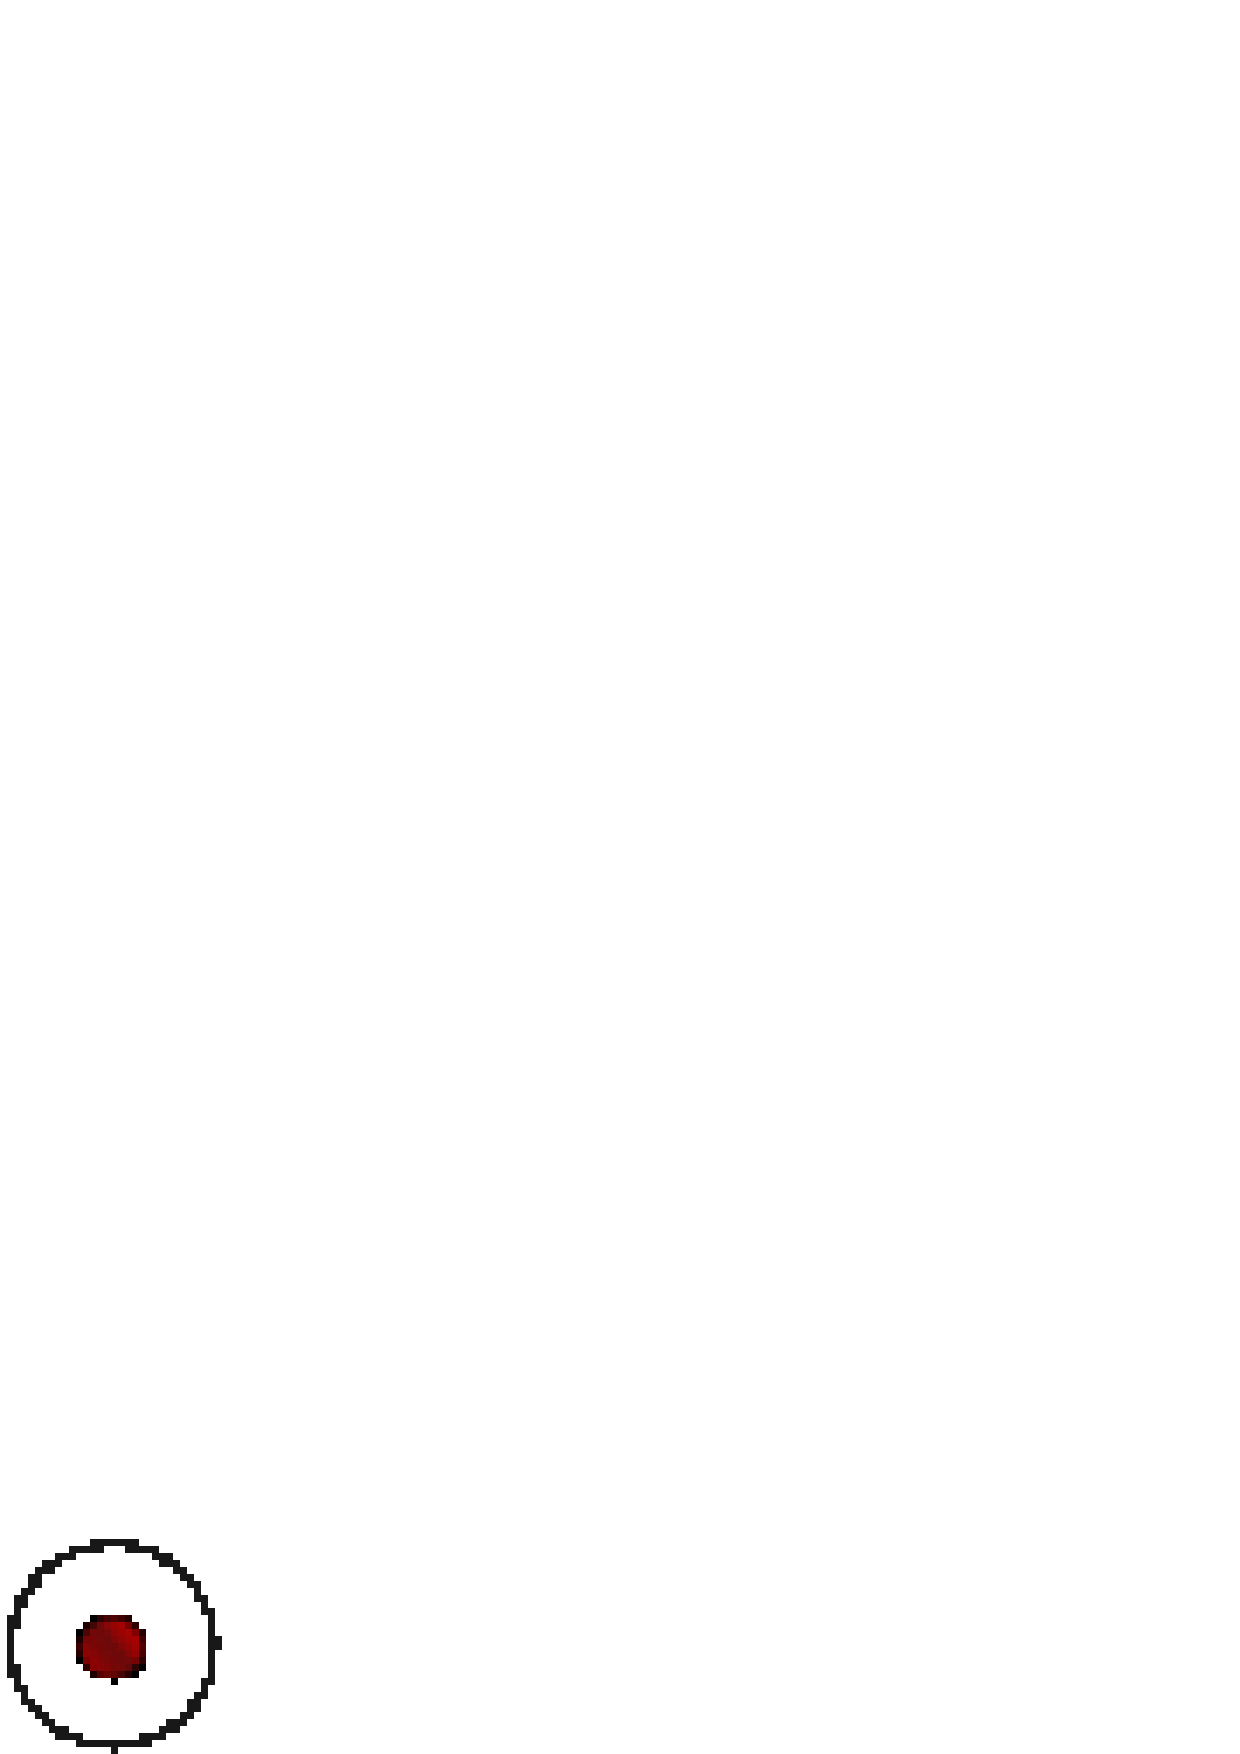
\includegraphics[width=0.7cm]{grass_new_centroid} & New Centroid & digitize new centroid (label existing area)\\
\hline 
\includegraphics[width=0.7cm]{grass_move_vertex} & Move vertex & select one vertex of existing line or boundary and
identify new position\\
\hline 
\includegraphics[width=0.7cm]{grass_add_vertex} & Add vertex & add a new vertex to existing line\\
\hline 
\includegraphics[width=0.7cm]{grass_delete_vertex} & Delete vertex & delete one vertex from existing line (confirm selected
vertex by another click)\\
\hline 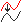
\includegraphics[width=0.7cm]{grass_move_line} & Move line & select existing line and click on new position\\
\hline 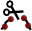
\includegraphics[width=0.7cm]{grass_split_line} & Split line & split an existing line to 2 parts\\
\hline 
\includegraphics[width=0.7cm]{grass_delete_line} & Delete line & delete existing line (confirm selected line by another
click)\\
\hline 
\includegraphics[width=0.7cm]{grass_edit_attributes} & Edit attributes & edit attributes of existing element (note that one
element can represent more features, see above)\\
\hline 
\includegraphics[width=0.7cm]{grass_close_edit} & Exit & close digitizing session (rebuilds topology afterwards)\\
\hline
\end{tabular}
\end{table}

\subsubsection{Category Tab}\index{GRASS!category settings}

This tab allows you to set the way in which the category will be assigned to
each new feature and/or assign a category to a feature.

\begin{itemize}
\item Mode: what category should be attached to geometry
\begin{itemize}
\item Next not used - next category not yet used in vector file
\item Manual entry - define the category in the 'Category'-entry field
\item No category - digitize geometry without entering any category
\end{itemize}
\item Category - a number (ID) attached to digitized feature
\item Field (layer) - feature (attribute table) identification
\end{itemize}

\begin{Tip}\caption{\textsc{Creating additional 'layers' with QGIS}}
\qgistip{If you would like to add more layers to your dataset, just add a new
number in the 'Field (layer)' entry box and press return. In the Table tab
you can create your new table connected to your new layer.
}
\end{Tip}

\subsubsection{Settings Tab}\label{label_settingtab}\index{GRASS!snapping
tolerance}

This tab allows you to set the snapping in screen pixels. This is the threshold
in pixels in which new points or line ends are snapped to existing nodes. This
helps prevent gaps or dangles between boundaries. The default is set to 10 
pixels.

\subsubsection{Symbology Tab}\index{GRASS!symbology settings}

This tab allows you to view and set symbology and color settings for various geometry types and
their topological status (e.g. closed / opened boundary).

\subsubsection{Table Tab} \index{GRASS!table editing}
This tab provides information about the database table for
a given 'layer'. Here you can add, modify or create new database tables for the
current layer.

\begin{Tip}\caption{\textsc{GRASS Edit Permissions}}\index{GRASS!edit
permissions}
\qgistip{You must be the owner of the GRASS mapset you want to edit. It is
impossible to edit vectors in mapsets which are not yours, even if you have
write permissions.
}
\end{Tip} 

\subsection{Region Tool}\index{GRASS!region}


\includegraphics[width=0.7cm]{grass_region_edit} The current region (window) in GRASS is very important for all 
raster modules. All newly-created rasters have the extension and resolution
of the current region, regardless of their original region. 
The region is stored in \$LOCATION/\$MAPSET/WIND file, and it defines
north, south, east, west, number of columns, number of rows, 
horizontal and vertical spatial resolution.

It is possible to switch on/off the GRASS region in the QGIS canvas
using the \textsl{Display Current GRASS Region}
button. \index{GRASS!region!display}

With the \textsl{Edit Current GRASS Region} you can open a tool 
in which you can change the current region and symbology
of the GRASS region rectangle on the QGIS canvas. When the tool is running,
it is also possible to select a new region interactively with your mouse
on the QGIS canvas.\index{GRASS!region!editing}

% Both tools are available only if QGIS has the GRASS-plugin enabled. 
% was started from a GRASS 
% shell or if the GISRC environment variable pointing to a
% valid GISRC file was set (i.e. only if you are running 
% GRASS within your mapset).

\subsection{GRASS Toolbox}\index{GRASS!toolbox}

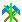
\includegraphics[width=0.7cm]{grass_tools} The GRASS toolbox provides 
analytic functions from GRASS within QGIS. To
use the GRASS toolbox you need to have opened a mapset where you have
write-permission. This is needed because QGIS will most probably create
new datasets which need to be written to a valid mapset.

Therefore you need to start QGIS from within a GRASS session. Then your 
current mapset will be opened for writing.

Another option for opening a mapset for writing is provided through the 
GRASS plugin entry. Use Plugins->GRASS->Open mapset.
 
If you have a greyed out GRASS toolbox button, make sure you open a valid
mapset for writing, since the GRASS plugin needs a mapset to store its
results.

The toolbox also provides a very useful data browser for browsing through your
current location and the mapsets it contains.


\subsubsection{Modules inside the toolbox} \index{GRASS!toolbox!modules}

The GRASS toolbox provide a collection of GRASS modules which can be used
from within QGIS. They are grouped in thematic blocks which can be defined 
by the user (see Section \ref{sec:toolbox-customizing}). 

When clicking on a module a new tab will be added to your toolbox which
provides three new sub-tabs:
\begin{enumerate}
\item Options
\item Output 
\item Manual
\end{enumerate}

\minisec{Options}

This tab provides you with a very simplified entry field where you need to 
select the needed maps and enter parameters to run the selected module.
Note, that these options are kept as simple as possible in order to keep
the structure clear. If you need more of the module's options, feel free to 
use the GRASS shell to run the module.

\minisec{Output}

This tab provides you with the output generated from the running module. After you hit the 
'run' button, the module switches to the Output-tab and you will see information about 
the process. If all goes well, you will see \texttt{Successfully finished} at the end.

\minisec{Manual}

This tab shows the help page of each GRASS module. You can have a look at the manual-page
if you want to get a deeper knowledge about the purpose of the module.
You may have recognized that some modules have more options and parameters than given in
the 'Options' tab. This is correct and done by design. To keep the GUI simple as possible
only the needed options and parameters are put in the Options tab. But you can always 
use the GRASS shell to run the module with all its parameters.

\begin{Tip}\caption{\textsc{Display results immediately}}\index{GRASS!display results}
\qgistip{If you want to display your calculation results immediately in your map canvas,
you can use the 'View Output' button at the bottom of the module tab.
}
\end{Tip} 


\subsubsection{GRASS Browser} \index{GRASS!toolbox!Browser}

Another useful feature is the GRASS browser. In Figure~\ref{subfig:grass_browser}
you can see the current location with its mapsets. 

The browser on the left allows you to browse through all your mapsets inside your selected
location. 

The right side of the browser window shows some meta information for the selected dataset, e.g. resolution,
bounding box, data source, attribute table for vector data\dots

The toolbar inside the browser tab gives you the following tools for the selected dataset:
\begin{itemize}
\item 
\includegraphics[width=0.7cm]{grass_add_map} Add selected map to canvas
\item 
\includegraphics[width=0.7cm]{grass_copy_map} Copy selected map
\item 
\includegraphics[width=0.7cm]{grass_rename_map} Rename selected map
\item 
\includegraphics[width=0.7cm]{grass_delete_map} Delete selected map
\item 
\includegraphics[width=0.7cm]{grass_set_region} Set current region to selected map
\item 
\includegraphics[width=0.7cm]{grass_refresh} Refresh browser window
\end{itemize}

The 'Rename' and 'Delete' buttons are only available in your current mapset. All other tools also work on
maps from other mapsets as well.

% Picture from the GRASS-Browser here:
\begin{figure}[h]
\centering
	\caption{GRASS toolbox}
   \subfigure[GRASS browser inside the toolbox]{\label{subfig:grass_browser}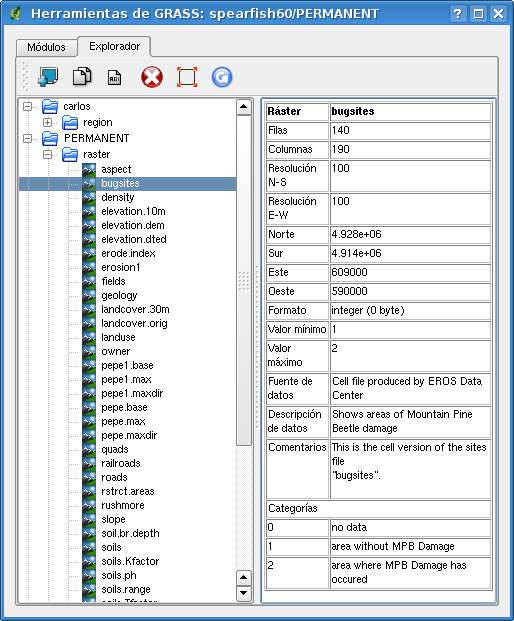
\includegraphics[clip=true, width=0.4\textwidth]{grassbrowser}}\goodgap
   \subfigure[GRASS shell inside the toolbox]{\label{subfig:grass_shell}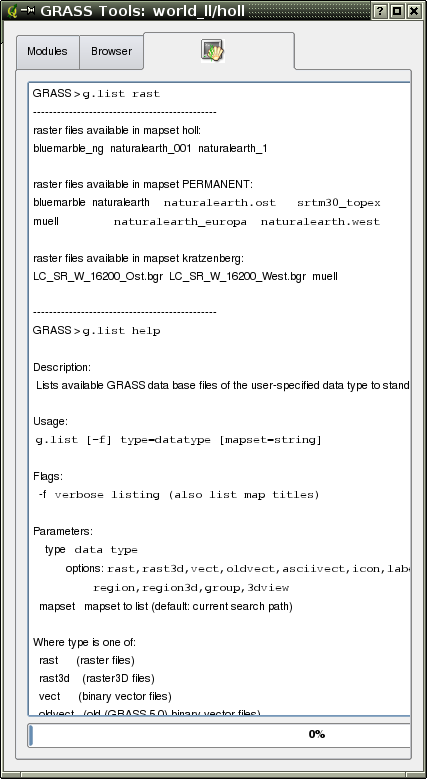
\includegraphics[clip=true, width=0.4\textwidth]{grassshell}}
\end{figure}

\subsubsection{Customizing the modules section} \index{GRASS!toolbox!customize}
\label{sec:toolbox-customizing}

Nearly all GRASS modules can be adopted to the GRASS toolbox. A XML interface is provided to parse
the very simple XML files which configure the modules inside the toolbox.

% TODO: migrating the content of this wiki-page into the manual?
A brief description of adding new modules, changing the modules group, etc. can be found on the QGIS wiki
at \url{http://wiki.qgis.org/qgiswiki/Adding\_New\_Tools\_to\_the\_GRASS\_Toolbox}.

A sample XML file for generating the module \texttt{v.buffer} (v.buffer.qgm) looks like this:
\begin{verbatim}
<?xml version="1.0" encoding="UTF-8"?>
<!DOCTYPE qgisgrassmodule SYSTEM "http://mrcc.com/qgisgrassmodule.dtd">

<qgisgrassmodule label="Vector buffer" module="v.buffer">
        <option key="input" typeoption="type" layeroption="layer" />
        <option key="buffer"/>
        <option key="output" />
</qgisgrassmodule>
\end{verbatim}

\begin{figure}[ht]
\centering
\caption{Module generated through parsing the XML-file}\label{fig:buffer-module}
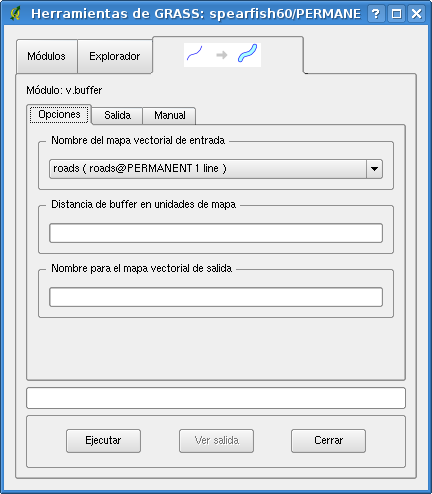
\includegraphics[clip=true, width=0.45\textwidth]{vbuffer}
\end{figure}

The parser reads this definition and creates a new tab inside the toolbox when you select 
the module:


\subsection{Creating a new GRASS layer}\label{sec:creating_new_grass_vectors}\index{GRASS!Creating new vectors|see{editing!creating a new layer}}

With this version of QGIS it is also possible to create new vectors from within GRASS very
easily.

Just select \textsl{Plugins->GRASS->Create new GRASS layer} from the toolbar, give a new name
in the text box and start digitizing.
If you encounter a greyed-out button, make sure you have a working mapset enabled. If you forgot
how to enable a mapset have a look at Section \ref{sec:load_grassdata}.

Since GRASS is able to organize all sort of geometries in one layer, there is no need to select
the geometry. This only applies to shapefile creation (see sec. \ref{sec:create shape}).

Some hints to make your digitizing more useful:
\begin{itemize}
\item Make sure to create an attribute table with its needed columns before you start digitizing
if you would like to assign attributes to your digitized object. 
Go to the table tab inside the digitize window.
\item If you plan to create a polygon layer, consider setting the mode to \textsl{No category}. 
Then start digitizing the boundaries which actually do not need an entry in the attribute table. 
If you have done this, change back to \textsl{Next not used} and start digitizing the centroids, which 
hold the attribute information of a polygon.

\end{itemize}

%\section{The GRASS Toolbar}
%The GRASS toolbar is displayed when the GRASS plugin is loaded using the
% Plugin Manager (see Section \ref{sec:managing_plugins}, \textsl{Managing
% Plugins}). Figure  shows the toolbar with each function annotated.
